\documentclass[11pt]{article}

% Paquetes
%===================================================================================================

% Establecemos los márgenes
\usepackage[a4paper, margin=1in]{geometry}

% Separacion entre parrafos
\setlength{\parskip}{1em}

% Paquete para incluir codigo
\usepackage{listings}

% Paquete para incluir imagenes
\usepackage{graphicx}
\graphicspath{ {./imagenes/} }

% Para fijar las imagenes en la posicion deseada
\usepackage{float}

% Para que el codigo acepte caracteres en utf8
\lstset{literate=
  {á}{{\'a}}1 {é}{{\'e}}1 {í}{{\'i}}1 {ó}{{\'o}}1 {ú}{{\'u}}1
  {Á}{{\'A}}1 {É}{{\'E}}1 {Í}{{\'I}}1 {Ó}{{\'O}}1 {Ú}{{\'U}}1
  {à}{{\`a}}1 {è}{{\`e}}1 {ì}{{\`i}}1 {ò}{{\`o}}1 {ù}{{\`u}}1
  {À}{{\`A}}1 {È}{{\'E}}1 {Ì}{{\`I}}1 {Ò}{{\`O}}1 {Ù}{{\`U}}1
  {ä}{{\"a}}1 {ë}{{\"e}}1 {ï}{{\"i}}1 {ö}{{\"o}}1 {ü}{{\"u}}1
  {Ä}{{\"A}}1 {Ë}{{\"E}}1 {Ï}{{\"I}}1 {Ö}{{\"O}}1 {Ü}{{\"U}}1
  {â}{{\^a}}1 {ê}{{\^e}}1 {î}{{\^i}}1 {ô}{{\^o}}1 {û}{{\^u}}1
  {Â}{{\^A}}1 {Ê}{{\^E}}1 {Î}{{\^I}}1 {Ô}{{\^O}}1 {Û}{{\^U}}1
  {ã}{{\~a}}1 {ẽ}{{\~e}}1 {ĩ}{{\~i}}1 {õ}{{\~o}}1 {ũ}{{\~u}}1
  {Ã}{{\~A}}1 {Ẽ}{{\~E}}1 {Ĩ}{{\~I}}1 {Õ}{{\~O}}1 {Ũ}{{\~U}}1
  {œ}{{\oe}}1 {Œ}{{\OE}}1 {æ}{{\ae}}1 {Æ}{{\AE}}1 {ß}{{\ss}}1
  {ű}{{\H{u}}}1 {Ű}{{\H{U}}}1 {ő}{{\H{o}}}1 {Ő}{{\H{O}}}1
  {ç}{{\c c}}1 {Ç}{{\c C}}1 {ø}{{\o}}1 {å}{{\r a}}1 {Å}{{\r A}}1
  {€}{{\euro}}1 {£}{{\pounds}}1 {«}{{\guillemotleft}}1
  {»}{{\guillemotright}}1 {ñ}{{\~n}}1 {Ñ}{{\~N}}1 {¿}{{?`}}1 {¡}{{!`}}1
}

% Para que no se salgan las lineas de codigo
% Para fijar una fuente que resalte
\lstset{breaklines=true, basicstyle=\ttfamily}

% Para que los metadatos que escribe latex esten en español
\usepackage[spanish]{babel}
\decimalpoint % Para que no se cambie el punto a la coma

% Para la bibliografia
% Sin esto, los enlaces de la bibliografia dan un error de compilacion
\usepackage{url}

% Para que se puedan clicar los enlaces
\usepackage{hyperref}

% Para mostrar graficas de dos imagenes, cada una con su caption, y con un caption comun
\usepackage{subcaption}

% Simbolo de los numeros reales
\usepackage{amssymb}

% Para que los codigos tengan una fuente distinta
\usepackage{courier}

\lstdefinestyle{CustomStyle}{
  language=Python,
  numbers=left,
  stepnumber=1,
  numbersep=10pt,
  tabsize=4,
  showspaces=false,
  showstringspaces=false
  basicstyle=\tiny\ttfamily,
}

% Para referenciar secciones usando el nombre de las secciones
\usepackage{nameref}

% Para enumerados dentro de enumerados
\usepackage{enumitem}

% Para mejores tablas
\usepackage{tabularx}

% Para poder tener el mismo identificador en dos tablas separadas
\usepackage{caption}

% Mostrar la página de las referencias en el indice del documento
\usepackage[nottoc,numbib]{tocbibind}

% Para mostrar las matrices
\usepackage{amsmath}

% Para que las notas al pie de pagina queden bien abajo
\usepackage[bottom]{footmisc}

% Comandos personalizados
%===================================================================================================

% Para realizar las citas de forma corta
\newcommand{\customcite}[1]{\emph{"\ref{#1}. \nameref{#1}"}}

% Para entrecomillar un texto
\newcommand{\entrecomillado}[1]{\emph{``#1''}}

% Metadatos del documento
%===================================================================================================
\title{
    {Inteligencia de Negocio - Práctica 2} \\
    {Análisis Relacional mediante Segmentación}
}

\author{
    {Sergio Quijano Rey - 72103503k}\\
    {sergioquijano@correo.ugr.es} \\
    {5º Doble Grado Ingeniería Informática y Matemáticas} \\
    {Grupo de prácticas 1}
}

\date{\today}

% Separacion entre parrafos
\setlength{\parskip}{1em}

% Contenido del documento
%===================================================================================================
\begin{document}

% Portada del documento
\maketitle
\pagebreak

% Indice de contenidos
\tableofcontents

% Lista de figuras
% Uso el addtocontents para que no se muestre la seccion de indice de figuras en el indice inicial

\addtocontents{toc}{\setcounter{tocdepth}{-10}}
\listoffigures

% TODO -- no tenemos cuadros en esta memoria
% \listoftables

% TODO -- tampoco tenemos codigos de relevancia
% \lstlistoflistings
\addtocontents{toc}{\setcounter{tocdepth}{3}}

\pagebreak

\section{Introducción}

\subsection{Problema a resolver}

En esta práctica, trabajaremos con un conjunto de datos del \entrecomillado{Instituto Nacional de Estadística}. En concreto, trabajamos con la \entrecomillado{Encuesta de condiciones de vida, 2020} \cite{original_dataset:online}. En términos del \entrecomillado{INE}, trabajamos con microdatos, lo que nos va a permitir realizar estudios en profundidad sobre la encuesta estudiada, más allá de los resúmenes basados en el estudio de las frecuencias, clásicos de las encuestas.

\subsection{Resumen de la forma de proceder}

Aunque más adelante, en el desarrollo de cada caso de estudio, se haga claro el procedimiento considerado, lo resumimos aquí de forma previa.

En cada caso de estudio, empezaremos definiendo el filtro que fija el caso de estudio en sí. Esto es, definimos la condición que filtrará las filas de nuestro conjunto de datos que estudiamos. Además, definimos las variables que consideramos, es decir, definimos las columnas del \emph{dataset} que consideramos para este caso de estudio.

Realizamos un procesado básico de los datos (borrado de datos faltantes, datos \lstinline{NaN}, borrado de \emph{outliers} y normalización). A partir de este procesado, realizamos cierto análisis exploratorio de datos, para tomar ideas a la hora de atacar cada problema en concreto.

A continuación, aplicamos los algoritmos de \emph{clustering}, mostrando gráficamente el resultado obtenido. Una vez ejecutados todos los algoritmos, calculamos un conjunto de métricas sobre los etiquetados generados, para poder comparar los resultados de los algoritmos. Visualizamos estas métricas y proyecciones del etiquetado a un espacio bidimensional (usando \emph{PCA} y \emph{tsne}).

Seguidamente, exploramos los parámetros de un par de algoritmos por cada caso de estudio, en busca de encontrar unos parámetros optimales para realizar la \emph{clusterización}.

Para finalizar, en esta memoria realizamos unas conclusiones, tanto del comportamiento de los algoritmos empleados como del conocimiento extraído sobre el conjunto de datos, gracias a las técnicas que hemos empleado.

\subsection{Observaciones y secciones previas}

Todo el código lo hemos organizado en un único \emph{Notebook} de \emph{Jupyter}. Para mantener el orden, hemos agrupado el código en secciones y subsecciones. Se puede explorar cómodamente esta jerarquía empleando \emph{Jupyter Lab} en vez de \emph{Jupyter Notebook}, o directamente empleado \emph{Google Colab}.

Hemos desarrollado una \textbf{sección inicial} con funcionalidades que vamos a estar usando durante todo el \emph{notebook}, evitando así repetir excesivamente el mismo código. Además, con esto, en las secciones de los casos de estudio nos centramos más en plantear ideas y ver los resultados, evitando toda la suciedad que supondría colocar en medio de estos desarrollos todo el código con la implementación. Esta sección previa de código común se divide en las siguientes subsecciones:

\begin{enumerate}
    \item Un decorador de \lstinline{Python} para poder medir fácilmente, y sin complicar el código, las funciones que calculan los \emph{clusters}. Esto es básico pues es una métrica que debemos estudiar, y que las librerías que estamos usando (principalmente \lstinline{sklearn}), no nos aportan de forma fácil
    \item Funciones para calcular \emph{clusters}. Destaca la función \lstinline{add_clustering_labels}, que toma como parámetro una función de clusterización con sus parámetros, y se encarga de calcular la clusterización y añadir las etiquetas al \lstinline{dataframe} convenientemente. Además, podemos especificar qué columnas ignorar en el \lstinline{dataframe} a la hora de calcular la clusterización (para no usar columnas con etiquetas de otros algoritmos, principalmente)
    \item Funciones para evaluar \emph{clusters}. En esta subsección definimos unas cuantas métricas que usaremos para comparar los resultados. La función \lstinline{compute_clustering_metrics} agrupa todas estas métricas y las devuelve convenientemente en un diccionario de \lstinline{Python}.
    \item Funciones para realizar visualizaciones. Con esto es más fácil usar las funciones de \lstinline{seaborn}, evitando tener que repetir código para, por ejemplo, excluir ciertas columnas del \lstinline{dataframe}. Destaca la función \lstinline{plot_centroids_with_size}. En esta función:
    \begin{itemize}
        \item Calculamos con código propio, por cada \emph{cluster}, el centroide y el radio de este, y el número de elementos en cada \emph{cluster}
        \item Aplicamos \emph{tsne} como técnica de proyección en un espacio bidimensional de los datos de entrada
        \item Con esta proyección, mostramos gráficamente los centroides obtenidos en la \emph{clusterización}, con un tamaño proporcional al radio previamente calculado, y con un color proporcional al número de elementos de cada \emph{cluster}
    \end{itemize}
    \item Funciones para procesar los \emph{dataframes}. Con esto, evitamos repetir el código que normaliza los datos, borra datos \lstinline{NaN} y borra \emph{outliers}
\end{enumerate}

Antes de pasar a los casos de estudio, debemos comentar otras dos secciones, la sección de filtrado previo del \emph{dataset} global y la sección de variables añadidas.

En la \textbf{sección de filtrado previo del \emph{dataset} global}, definimos el conjunto de variables que nos interesan, descartando el resto por completo. Esta selección se realizó al principio del desarrollo de la práctica, buscando una primera exploración del conjunto de datos. Por esto se seleccionan variables que más tarde no se usan para nada. Pero decidimos dejar estas variables en el \emph{Notebook}  como ilustración de cuál fue nuestro proceso a la hora de abordar el problema. Nos quedamos, en esta fase, con un total de \textbf{39 variables}.

En la \textbf{sección de variables añadidas}, definimos algunas variables agregadas (que combinan información de varias variables, o que transforman la información en bruto) a nuestro \emph{dataset}. En concreto:

\begin{itemize}
    \item Definimos la variable \lstinline{booleana} \lstinline{pidio_ayuda} que controla si un hogar pidió o no pidió ayuda, ya sea a un familiar o a otro tipo de entidad.
    \item Definimos la variable \lstinline{gasto_transporte_total} que combina el gasto en transporte público y transporte privado
    \item Definimos la variable \lstinline{retraso_pago}, que controla si se produjo cualquier tipo de retraso en los pagos
    \item Definimos la variable \lstinline{ingresos_menos_gastos}, que realiza la resta de todos los ingresos de un hogar menos todos los gastos, registrados en el \emph{dataset}, de ese hogar
    \item Definimos la variable ordinal \lstinline{comunidad_autonoma_code}, que convierte el código en texto de una comunidad autónoma a una variable entera. Esto con la intención de poder usar esta variable en los algoritmos de \emph{clusterización}
    \item Definimos la variable \lstinline{habitaciones_por_persona} que calcula el cociente del número de integrantes de un hogar entre el número de habitaciones de dicho hogar
\end{itemize}

Con todo esto, pasamos a tener un total de \textbf{45 variables}. De nuevo, algunas de estas variables añadidas no se usan en los casos de estudio, pero las dejamos para ilustrar el proceso realizado en la búsqueda de casos de estudio interesantes.

A partir de este punto ya nos encontramos con las secciones propias a los casos de estudio, que pasamos a comentar en cada sección correspondiente.

\pagebreak

\section{Caso de estudio 1}

\subsection{Definición del caso de estudio}

En este caso de estudio queremos poner nuestra atención en aquellas personas que \textbf{viven en un entorno en el que hay vandalismo}. Para ello usamos la variable \lstinline{vandalismo_en_la_zona}, que se corresponde con el código \lstinline{"HS190"}.

Una vez filtradas las filas que vamos a estudiar, filtramos las variables (columnas) que nos interesan. En concreto, nos quedamos con la renta disponible del hogar, los gatos mensuales de la vivienda, el gasto total en transporte y los códigos de la comunidad autónoma. Nos interesa realizar los siguientes estudios:

\begin{itemize}
    \item Estudiar la distribución del vandalismo por cada comunidad autónoma
    \item Estudiar el uso del transporte en las zonas conflictivas
    \item Lógicamente, nos interesa el factor económico involucrado en definir zonas posiblemente conflictivas. La hipótesis básica es que en las zonas de menor renta hay más vandalismo. Pero también puede haber vandalismo en las zonas más pudientes (robos, asaltos a casas, \ldots)
    \item El gasto en vivienda puede ser interesante como otra variable para fijar el estatus socio-económico. En ciertas comunidades autónomas, un alto gasto en vivienda no significa un nivel alto de vida (precios demasiado inflados, precios en zonas urbanas mucho más altos que en zonas rurales, \ldots)
\end{itemize}

Además, en el \emph{dataframe} que usamos para almacenar estos datos (\lstinline{df_study_case}), guardamos el factor de elevación, que usaremos para ponderar los ejemplos, en aquellos algoritmos que acepten este parámetro de ponderación.

Tras el filtrado, obtenemos un \emph{dataset} con 2081 filas (objetos a \emph{clusterizar}) y 5 columnas (4 + 1 para el factor de elevación).

\subsection{Procesado de los datos}

Como ya hemos comentado previamente, realizaremos el siguiente pre-procesado de los datos:

\begin{itemize}
    \item Borrado de las filas que contengan algún valor \lstinline{NaN}
    \item Borrado de \emph{outliers} usando la regla $3 \cdot IQR$, variable por variable
    \item Normalización del rango de las variables al intervalo $[0, 1]$
\end{itemize}

Tras aplicar esto, nos quedamos con un \emph{dataset} de 1947 filas.

\subsection{Análisis Exploratorio de datos}

Comenzamos haciendo un \emph{plot} por pares de variables, que mostramos en la siguiente figura:

\begin{figure}[H]
    \centering

    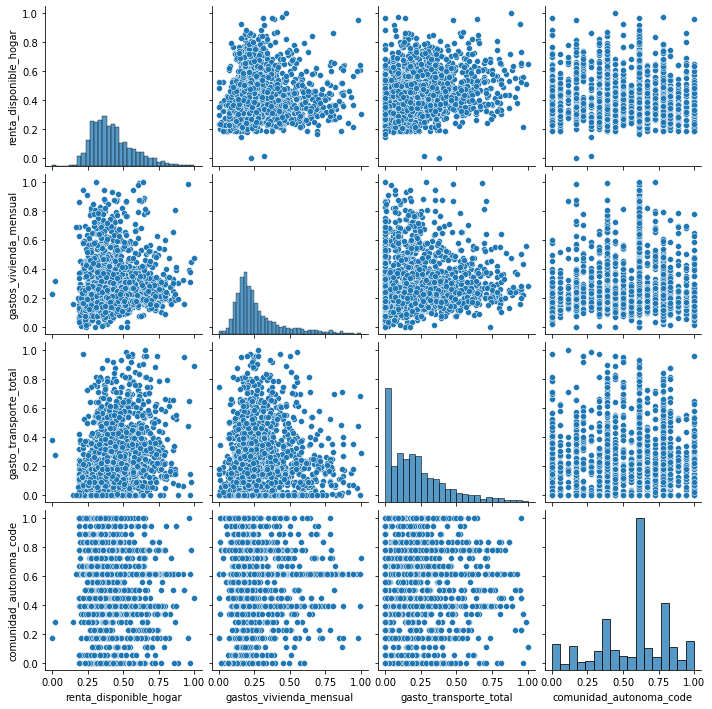
\includegraphics[width = 0.9 \textwidth]{stcase01_pairplot}
    \caption{Gráfico en el que se muestran todas las combinaciones de parejas de variables involucradas en el caso de estudio}
    \label{stcase01_pairplot:figura}
\end{figure}

En este gráfico tenemos las distribuciones al poner en un eje una variable y en el otro eje otra variable, considerando todas las parejas posibles. En la diagonal tenemos la distribución de cada variable, por sí sola.

Lo que más llama la atención de este gráfico es que, en la distribución de las comunidades autónomas, hay una comunidad que destaca claramente sobre otras. Esto podría ser porque dicha comunidad autónoma tiene una mayor representación en la encuesta, o no. Por tanto, es necesario visualizar dicha distribución de forma porcentual, considerando como base para el cálculo toda la población.

El resto de distribuciones tienen una forma parecida a la normal, lo que era de esperar. Salvo la distribución del gasto en transporte, donde el gasto mínimo (puede que no sea nulo, pues hemos normalizado las variables al rango $[0, 1]$) destaca sobre el resto de valores, rompiendo con una distribución normal que esperábamos.

Se puede apreciar cierta correlación positiva entre la renta disponible en el hogar y el gasto en vivienda mensual. Pero parece ser una correlación muy débil y que no destaca nada interesante (es lógico que a mayor dinero disponible, generalmente se gaste más en vivienda).

La correlación entre gasto en vivienda y gasto en transporte no parece aportar nada nuevo al estudio que queremos realizar.

Por la naturaleza ordinal del código de la comunidad autónoma, no podemos extraer mucha información al respecto usando esta gráfica y esta variable en concreto.

Como comentábamos previamente, destaca los picos de ciertas comunidades autónomas en el número de hogares que viven en un entorno de vandalismo. Pero esto puede deberse a diferencias en tamaños de las comunidades. Así que pasamos a mostrar el porcentaje de hogares que viven en entornos con vandalismo, agrupados por comunidades autónomas:

\begin{figure}[H]
    \centering

    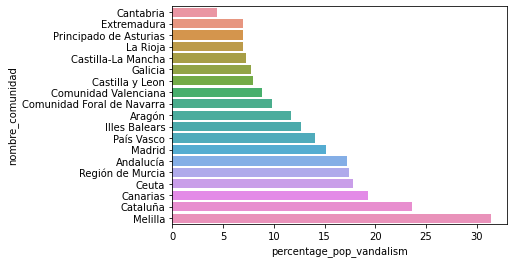
\includegraphics[width = 0.8 \textwidth]{stcase01_porcentajes_vandalismo}
    \caption{Gráfico con el porcentaje de hogares que viven en entornos con vandalismo, agrupados por comunidades autónomas}
\end{figure}

En este gráfico podemos ver que, como suponíamos, hay ciertas comunidades autónomas con un porcentaje de hogares en zonas con vandalismo mucho mayores que otras comunidades. Destaca la ciudad autónoma de Melilla, que se distancia de la segunda peor comunidad en esta métrica prácticamente un 10\%. Además, a la vista de estos datos, y sin necesidad de introducir datos externos sobre poblaciones de las comunidades autónomas, parece que las zonas más rurales y con menos concentración de población (Cantabria, Extremadura, Asturias, \ldots) tienen porcentajes de vandalismo significativamente mayor que comunidades más densamente pobladas (Cataluña, Andalucía, Madrid, \ldots). Destacan, saliéndose de lo que acabamos de comentar, las dos ciudades autónomas.

Aprovechamos la sección de exploración de datos de este caso de estudio para realizar la siguiente observación, que tendrá impacto en el resto de casos de estudio. En un primer momento, consideramos usar las variables \lstinline{renta_disponible_total_hogar} y \lstinline{renta_disponible_restado_alquiler}. Sin embargo, como mostramos a continuación, están muy correladas, por lo que no aportan información interesante:

\begin{figure}[H]
    \centering

    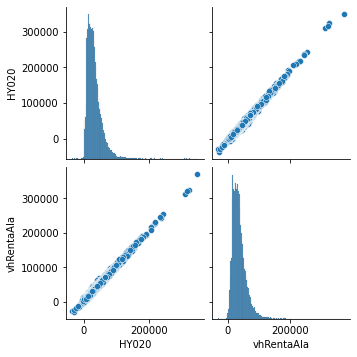
\includegraphics[width = 0.6 \textwidth]{stcase01_correlacion_renta_total_restado}
    \caption{Gráfico en el que se aprecia claramente la correlación entre la variable \lstinline{renta_disponible_total_hogar} y la variable \lstinline{renta_disponible_restado_alquiler}}
\end{figure}

Lo mismo ocurre con la variable agregada por nosotros, \lstinline{ingresos_menos_gastos}, y la variable ya presente en los datos originales, \lstinline{renta_disponible_total_hogar}. Esto se muestra claramente en la siguiente gráfica:

\begin{figure}[H]
    \centering

    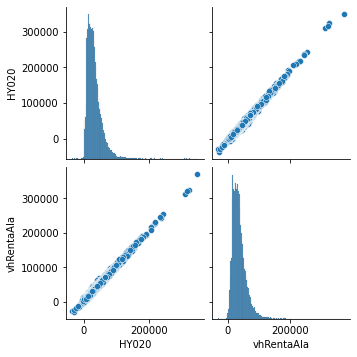
\includegraphics[width = 0.6 \textwidth]{stcase01_correlacion_renta_total_mi_variable_agregada}
    \caption{Gráfico en el que se aprecia claramente la correlación entre la variable \lstinline{renta_disponible_total_hogar} y la variable agregada \lstinline{renta_disponible_restado_alquiler}}
\end{figure}

Por tanto, no tiene sentido usar ambas variables en un mismo caso de estudio, pues apenas aportan información nueva al problema, debido a la alta correlación entre ambas.


\subsection{Resultados de \emph{clustering}}

\subsection{Interpretación de la segmentación}

% TODO -- poco gasto en transporte, como muestra \ref{stcase01_pairplot:figura}

\pagebreak

\section{Caso de estudio 2}

\pagebreak

\section{Caso de estudio 3}

\pagebreak

% Bibliografia
\bibliography{./References}
\bibliographystyle{ieeetr}

\end{document}
